Alur, Madhusudan 2004 / Mehlhorn 1980 (input driven PDA)
\section{Motivation}
    \begin{itemize}
        \item Tradeoff: Ausdrucksstärke vs. Abschlusseigenschaften, Entscheidbarkeit
        \item guter Tradeoff: VPL
        \item PDA (Kellerautomat): Akzeptiert per leerem Keller
        \item DPDA (deterministischer Kellerautomat): Akzeptiert per Endzustand
        \item VPA ist eingeschränkter DPDA:
        \begin{itemize}
            \item Eingabezeichen bestimmen Kelleraktion
            \item Partitionierung des Alphabets:
            \subitem $\Sigma=\Sigmapush\dcup\Sigmapop\dcup\Sigmaneut$
            \subitem $\Sigmah=\left(Sigma_{push},\Sigmapop,\Sigmaneut\right)$
            \subitem push = call, pop = return, neutral = internal
        \end{itemize}
        \item Beispiel: $\Sigmah=\left(\{a\},\{b\},\{c\}\right)$
        \begin{itemize}
            \item $a^nb^n$
            \item $(a^nb^n)^*$
            \item $\{w\mid|w|_a=|w|_b\}\not\in VPL$
            \subitem $\rightarrow$ bei negativem Keller nie in VPL
        \end{itemize}
        \item Denkmodell: $\Delta w=|w|_{\Sigmapush}-|w|_{\Sigmapop}$
        \subitem $\rightarrow$ hat \qq{Zacken}, muss am Ende des Wortes wieder bei 0 sein
    \end{itemize}
\section{Definition: PDA}
    $M=(Q,Q_S,Q_F,\Gamma,\Sigmah,\delta,\#)$ mit:
    \begin{itemize}
        \item $Q$: Zustände
        \item $Q_S$: Startzustände
        \item $Q_F$: Endzustände
        \item $\Gamma$: Kelleralphabet
        \item $\hat\Sigma$: Eingabealphabet
        \item $\#$: Kellerbodenzeichen
        \item $\delta$: Übergänge
        \subitem $\delta \subseteq Q\times \Sigmaneut \times Q \\\cup Q\times \Sigmapush \times \Gamma\setminus\{\#\}\times Q\\\cup Q\times \Sigmapop \times\Gamma\times Q$
    \end{itemize}
\section{Semantik}
    \begin{itemize}
        \item Konfiguration: Element $Q\times\Sigmah^*\times \Gamma^*$
        \item Konfigurationsübergänge: Relation $\rightarrow \subseteq K\times K$
        \item $c\in\Sigmaneut:\ q,w_1,\dots,w_n,\gamma_1,\dots,\gamma_k\rightarrow \delta(q,c),w_1,\dots,w_{n-1},\gamma_1,\dots,\gamma_k$
        \item $a\in\Sigmapush:\ q,w_1,\dots,w_n,\gamma_1,\dots,\gamma_k\rightarrow q',w_1,\dots,w_{n-1},\gamma_1,\dots,\gamma_k,\gamma$
        \subitem $(q',\gamma)\in\delta(q,a)$
        \item $b\in\Sigmapop:\ q,w_1,\dots,w_n,\gamma_1,\dots,\gamma_k\rightarrow q',w_1,\dots,w_{n-1},\gamma_1,\dots,\gamma_{k-1}$
        \subitem $q'\in\delta(q,b,\gamma_k)$
        \item $L(M):=\left\{w\mid\exists s\in Q_S\exists f\in Q_F: s,w,\# \rightarrow^* f,\varepsilon,\# \text{ oder } \in\Gamma^*\#\right\}$
    \end{itemize}
\section{Alur-Kongruenz}
\subsection{Wiederholung: Myhill-Nerode}
    Myhill-Nerode-Relation in Abhängigkeit von $L\subseteq \Sigma^*$\\
    $u\sim_L v :\Leftrightarrow \forall x,y: xuy\in L \Leftrightarrow xvy\in L$ (syntaktische Kongruenz)\\
    $\Sigma^*/\sim_L=\{[w]|w\in\Sigma^*\}$ heißt syntaktisches Monoid
    \subsubsection{Anmerkungen}
        \begin{itemize}
            \item $[w_1][w_2]=[w_1w_2]$
            \item L regulär $\Leftrightarrow |\Sigma^*/\sim_L|$ endlich
        \end{itemize}
\subsection{Definition}
    $u,v\in WM$ (WM: Well-matched $\rightarrow$ akzeptieren mit leerem Keller im Endzustand)\\
    $u\simeq v :\Leftrightarrow \forall x,y\in\Sigma^*: xuy\in L\Leftrightarrow xvy\in L$
\subsection{Satz}
    $L$ ist VPL $\Leftrightarrow |WM/\simeq |$ endlich
\subsection{Anmerkungen}
    \begin{itemize}
        \item Operationen
            \begin{itemize}
                \item Konkatenation
                \item Extend:
                \subitem $[w]\rightarrow [awb],\ a\in\Sigmapush,b\in\Sigmapop$
            \end{itemize}
        \item $WM:=\{w\in\Sigma^* \mid \Delta(w)=0\wedge \forall i\le|w|:\Delta(w_1\dots w_i)\geq 0\}$
        \subitem mit $\Delta(w)=|w|_{\Sigmapush}-|w|_{\Sigmapop}$
        \item $\Sigma^* \supseteq L$ regulär $\rightarrow \Sigmah=(\emptyset,\emptyset,\Sigma)$
        \item Jedes visibly Wort lässt sich durch concat und extend erzeugen
    \end{itemize}
    \subsubsection{Beispiel}
    \vspace*{2cm}Leite $aaabbabb$ ab:\vspace*{-2.5cm}\\
        \hspace*{5cm}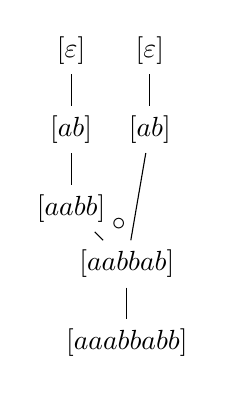
\begin{tikzpicture}
            \node (A) {$[\varepsilon]$};
            \node (Z) [right of=A] {$[\varepsilon]$};
            \node (B) [below of=A] {$[ab]$};
            \node (Y) [below of=Z] {$[ab]$};
            \node (C) [below of=B] {$[aabb]$};
            \node (D) [below right of=C] {$[aabbab]$}; \node[above of=D, yshift=-.5cm,xshift=-.1cm]{$\circ$};
            \node (E) [below of=D] {$[aaabbabb]$};
            \path (A) edge (B)
                (B) edge (C)
                (C) edge (D)
                (D) edge (E)
                (Z) edge (Y)
                (Y) edge (D);
        \end{tikzpicture}
\section{Satz}
    Für jeden VPA M existiert DVPA $M'$ mit L(M)=L($M'$) wobei L(M)$\subseteq$WM
    \subsubsection{Beweis}
    geg. $M=(Q,Q_S,Q_F,\Gamma,\Sigmah,\delta,\#)$, konstruiere $M'=(Q',q_S',Q_F',\Gamma',\Sigmah,\delta',\#)$
    \begin{itemize}
        \item $Q'=\mathcal{P}(Q\times Q)$
        \item $q_S'=\{(q,q)\mid q\in Q\}\in Q'$ (=$id_Q$)
        \item $Q_F'=\{S\in Q'\mid \exists s\in Q_S\exists f\in Q_F: (s,f)\in S\}$
        \item $\Gamma'=\Sigmapush\times Q'\cup \{\#\}$
        \item $\delta'$:
        \begin{itemize}
            \item $a\in\Sigmapush: \delta'(S,a)=(id_Q,(a,S))$
            \item $b\in\Sigmapop : \delta'(S,b,(a,S))=S''$\\%TODO: Formatting
            $S''=\{(q,q')\mid\exists q_1,q_2,q_3: (q,q_1)\in S', \exists\gamma\in\Gamma:(q_2,\gamma)\in\delta(q_1,a), (q_2,q_3)\in S, q'\in\delta(q_3,b,\gamma))\}$
            \item $c\in\Sigmaneut: \delta'(S,c)=\{(q,q')\mid \exists q''\in Q: (q,q'')\in S\wedge q'\in \delta(q'',c)\}$
        \end{itemize}
    \end{itemize}
\section{Satz von Chomsky-Schützenberger, 1963}
    Jede kontextfreie Sprache ist das homomorphe Bild einer Sprache $\mathds{D}_{2k}\cap R$ wobei $R$ regulär.\\
    $\forall L\subseteq \Sigma^*\text{ kf. }\exists k\in\mathds{N}, R\text{ reg. }\exists\varphi:L=\varphi(\mathds{D}_{2k}\cap R)$ $\varphi:\Sigma^*\rightarrow \{[_1,]_1,[_2,]_2,\dots\}^*$
    \subsection{Beweis}
        $L$ kf $\Rightarrow\exists G=(V,\Sigma,P,s)$ mit $L(G)=L$ und $L$ in CNF\\
        $X\in L(G)\Leftrightarrow\exists$ Ableitungsbaum (mit CNF: Binärbaum)\\
        Idee: Nutze Korrespondenz zwischen Bäumen und Dyck-Sprachen.\\\vspace{2mm}
        Konstruiere Grammatik $G'=(V',\Sigma',P',S')$ wobei $L(G')=\mathds{D}_{2k}\cap R$\\
        Sei $P=\{\Pi_1,\dots,\Pi_k\}$, dann $P'=\{\Pi_1',\dots,\Pi_k'\}$
        \begin{itemize}
            \item ist $\Pi_i=A\rightarrow BC$, dann $\Pi_i'=A\rightarrow\mathop{[}\limits_i^1B\mathop{]}\limits_i^1\mathop{[}\limits_i^2C\mathop{]}\limits_i^2$
            \item ist $\Pi_i=A\rightarrow a$, dann $\Pi_i'=A\rightarrow\mathop{[}\limits_i^1\mathop{]}\limits_i^1\mathop{[}\limits_i^2\mathop{]}\limits_i^2$
        \end{itemize}
        $\Sigma'=\{\mathop{[}\limits_i^1,\mathop{]}\limits_i^1,\mathop{[}\limits_i^2,\mathop{]}\limits_i^2,\dots,\mathop{[}\limits_k^1,\mathop{]}\limits_k^1,\mathop{[}\limits_k^2,\mathop{]}\limits_k^2\}$\\
        Wähle $\varphi:\Sigma'\rightarrow\Sigma$:
        \begin{itemize}
            \item Ist $\Pi_i=A\rightarrow BC$, so $\varphi(\mathop{[}\limits_i^1)=\varphi(\mathop{]}\limits_i^1)=\varphi(\mathop{[}\limits_i^2)=\varphi(\mathop{]}\limits_i^2)=\varepsilon$
            \item Ist $\Pi_i=A\rightarrow a$, so $\varphi(\mathop{]}\limits_i^1)=\varphi(\mathop{[}\limits_i^2)=\varphi(\mathop{]}\limits_i^2)=\varepsilon,\varphi(\mathop{[}\limits_i^1)=a$
        \end{itemize}
        \begin{enumerate}[1)]
            \item $L=\varphi(L(G'))$
            \item $L(G')=\mathds{D}_{2k}\cap R$
        \end{enumerate}
        \begin{enumerate}[1)]
            \item $x\in L \Leftrightarrow x\in L(G)\\\Leftrightarrow \exists$ Ableitungsbaum von G für $x\\\Leftrightarrow x'\in L(G'),$ wobei $x'$ Klammerrepräsentation des Baumes ist$\\\Leftrightarrow x\in\varphi(L(G'))$, da für jedes Blatt das richtige Zeichen übrig bleibt
            \item offensichtlich: $L(G')\subseteq\mathds{D}_{2k}$\\
            Weitere Bedingungen an die Wörter, um Konstruktion zu genügen:
            \begin{enumerate}[a)]
                \item einem $\mathop{]}\limits_i^1$ muss immer $\mathop{[}\limits_i^2$ folgen
                \item einem $\mathop{]}\limits_i^2$ muss $\mathop{]}\limits_j^1$ oder $\mathop{]}\limits_j^2$ folgen (beachte Sonderfall für Startvariable)
                \item ist $\Pi_i=A\rightarrow BC$, dann muss $\mathop{[}\limits_i^1$ ein $\mathop{[}\limits_p^1$ folgen mit $\Pi_p=B\rightarrow EF$ oder $\Pi_p=B\rightarrow b$ und $\mathop{[}\limits_i^2$ muss immer $\mathop{[}\limits_q^1$ folgen mit $\Pi_q=C\rightarrow GH$ oder $\Pi_q=C\rightarrow c$
                \item ist $\Pi_i=A\rightarrow a$, dann muss auf $\mathop{[}\limits_i^1$ $\mathop{]}\limits_i^1$ folgen und auf $\mathop{[}\limits_i^2$ $\mathop{]}\limits_i^2$ und auf $\mathop{]}\limits_i^1$ $\mathop{[}\limits_i^2$
                \item $\mathop{[}\limits_i^1$ als erstes Zeichen, dann muss $\Pi_i$ S auf der linken Seite haben
            \end{enumerate}
            \item[$\rightarrow$] Bedingungen sind alle regulär. Schneide alle Sprachen dieser Bedingungen; erhalte $R$, regulär.
        \end{enumerate}
\section{Satz von Greibach}
    \qq{Die schwerste kontextfreie Sprache}\\
    \subsection{Satz (Greibach, 1974)}
        Es gibt eine feste Sprache $L_0$, sodass $L$ kontextfrei $\Leftrightarrow \exists$ Homomorphismus $\varphi: L=\varphi^{-1}(L_0)$
        \subsubsection{Anmerkungen}
            \begin{itemize}
                \item Homomorphismen sind leicht zu berechnende Reduktionen
                \item Interpretation: Kann eine Maschine $L_0$ entscheiden, so auch jede andere kontextfreie Sprache
                \item $L$ kontextfrei $\Rightarrow\exists G:L=L(G),\ G$ in Greibachnormalform (GNF):
                \subitem $A\rightarrow aA_1A_2\dots A_k$
            \end{itemize}
        \subsubsection{Beweis}
            \emph{Idee:} Wähle $\varphi$ und $L_0$ so, dass sich Ableitung in GNF in $L_0$ wiederfindet.\\[0.2cm]
            $\Sigma=\{a_1,a_2,b_1,b_2,c,d,\$\},\ L_0\subseteq \Sigma^*,\ x_i,z_i\in\Sigma^*, y_1y_2\dots y_n\in\$\mathds{D}_2$\\
				$L_0 = \{\epsilon\}\{x_1cy_1cz_1d\dots x_0cy_ncz_nd| n\geq 1;x_i,z_i \in \Sigma^*; y_1,y_2,\dots,y_n\in \$\mathbb{D}_2$\\
            $L_0$ ist kontextfrei.\\[0,2cm]
            Sei G in GNF mit $L=L(G)$ und $G=\left(\{A_1,\dots,A_{|V|}\},\Gamma,P=\{\Pi_1,\dots,\Pi_k\},A_1\right),\ P_a=\{\Pi\in P\mid \Pi$ beginnt rechts mit $a\},\ \forall a\in\Gamma$\\
            $\varphi:\Gamma^*\rightarrow\Sigma^*, a\mapsto \left(\prod\limits_{\Pi\in P_a}c\Tau(\Pi)\right)cd=c\Tau(\Pi_{P_1})c\Tau(\Pi_{P_2})\dots c\Tau(\Pi_{|P_a|})cd$\\
            $\Pi_j=A_i\rightarrow aA_{j_1}\dots A_{j_m}$\\
            $\Tau(\Pi_j)=\underbrace{b_1b_2^ib_1}_{A_i}\underbrace{a_1a_2^{j_m}a_1}_{A_{j_m}}\dots \underbrace{a_1a_2^{j_1}a_1}_{A_{j_1}}$\\
            Sonderfall:\\
            $\Pi_j=a_1\rightarrow\dots \Rightarrow \Tau(\Pi_j)=\$a_1a_2^1a_1\Tau(\Pi_j)$ (wie oben)\\
            Anm: Startvariable kommt nur links vor
        \subsubsection{Beispiel}
            \begin{align*}
                \Pi_1=A_1\rightarrow aA_2A_2 && \Tau(\Pi_1)=\$a_1a_2^1a_1b_1b_2^1b_1a_1a_2^2a_1a_1a_2^2a_1\\
                \Pi_2=A_2\rightarrow a && \Tau(\Pi_2)=b_1b_2^1b_1\\
                \Pi_3=A_2\rightarrow bA_2 && \Tau(\Pi_3)=b_1b_2^1b_1a_1a_2^2a_2\\
                \Pi_4=A_2\rightarrow b && \Tau(\Pi_4)=b_1b_2^1b_1
            \end{align*}
            $\varphi(a) = c\Tau(\Pi_1)c\Tau(\Pi_2)cd\\
            \varphi(b) = c\Tau(\Pi_3)c\Tau(\Pi_4)cd\\
            A_1\Rightarrow_G^* aabA_2$\\
            \begin{align*}
                \varphi(aab) =& c\Tau(\Pi_1)c\Tau(\Pi_2)cdc\Tau(\Pi_1)c\Tau(\Pi_2)cdc\Tau(\Pi_3)c\Tau(\Pi_4)cd\\
                =& c\$a_1a_2^1a_1b_1b_2^1b_1a_1a_2^2a_1a_1a_2^2a_1cb_1b_2^2b_1cd\\
                &c\$a_1a_2^1a_1b_1b_2^1b_1a_1a_2^2a_1a_1a_2^2a_1cb_1b_2^2b_1cd\\
                &cb_1b_2^2b_1a_1a_2^2a_1cb_1b_2^2b_1cd
            \end{align*}
            Ableitung $aabA_2$:\\
            $$A_1\overset{\Pi_1}{\Rightarrow}aA_2A_2\overset{\Pi_2}{\Rightarrow}aaA_2\overset{\Pi_3}{\Rightarrow}aabA_2\dots$$
            $y_1y_2y_3$ \qq{kürzen}$\rightarrow \$a_1a_2^2a_1=\mu(y_1y_2y_3)$\\
            $y_4=\Tau(\Pi_4)\rightarrow y_1y_2y_3y_4\in\$\mathds{D}_2$
            Leite in Satzform immer die Variable am weitesten links ab.\\
            Allgemein:\\
            $(*) A_1'\rightarrow aB_1\dots B_m$\\
            $A_1\Rightarrow_G^* a_1\dots a_kA_1'\dots A_n \overset{(*)}{\Rightarrow} a_1\dots a_kaB_1\dots B_mA_2\dots A_n$\\
            $A_1\bar{A_1}\dots \mid A_n'\dots A_1'\leadsto A_n'\dots A_1'\bar{A_1'}B_m\dots B_1$
%TODO: 2015-11-10
	\\\\ wir zeigen:\\
	$S\Rightarrow_G^* a_1\dots a_kA_{i1}\dots A_{ir} \text{ mit Produktionen } (\Pi_{p1},\dots,\Pi_{pk})\\
	\Longleftrightarrow$\\
	\begin{enumerate}[(a)]
		\item $\varphi(a_1\dots a_k)=x_1c_{y1}c_{z1}d\dots x_kc_{yk}c_{zk}d$ \\\textit{$x_i$= nicht benutzte Produktionen ?}
		\item $y_1\dots y_k \in Prefix(\$\mathds{D}_2)$
		\item $\mu(y_1\dots y_k)= \$a_1a_2^{ir}a_1\dots a_1a_2^{i1}a_2$
	\end{enumerate}
	also $S\Rightarrow^* a_1\dots a_k \Leftrightarrow a) \cap y_1\dots y_n \in \$ \mathds{D}_2 \cap \mu(y_1\dots y_n)=\$$
\subsubsection{Beweis}durch Induktion über K\\
	
		IA:\\$ S\Rightarrow_G^1 a_1A_{i1}\dots A_{ir} \text{ dann }\\
		ex \Pi =S \rightarrow a_1A_{i1}\dots A_{ir} \in P_{a_1} \\
		\varphi(a_1)=x_1c_{y_1}c_{z_1}d= c\Tau(\Pi_{p1})c\Tau(\Pi_{p2})c\dots c \Tau(\Pi_{pm})d$\\\\
		$\Tau(\Pi)=\$a_1a_2a_1b_1b_2b_1a_1a_2^{ir}a_1\dots a_1a_2^{i1}a1$\\
		$	\rightarrow a) \checkmark b) \checkmark c)\checkmark$ offensichtlich.\\
		IS:  \\
		Induktions Annahme:\\
		$S\Rightarrow_G^*a_1\dots a_k A_{i1}\dots A_{ir} \Leftrightarrow a)\cap b) \cap c) \checkmark$\\
		sei $\Pi = A_{i1} \rightarrow a_{k+n} A_{j1}\dots A_{jt} \in P_a$ dann:\\
		$S \Rightarrow_G a_1\dots a_{k+1} % 1 oder n?
		A_{j1}\dots A_{jt}A_{i2}\dots A_{ir}$\\
		Induktiv:\\
		$\mu(y_1\dots y_k)=\$a_1a_2^{ir}a_1\dots a_1a_2^{i1}a_2\\
		\mu(y_1\dots y_k)\mu(y_{k+1})=\$a_1a_2^{ir}a_1\dots \cancel{a_1a_2^{i1}a_2} \cancel{b_1b_2^{i1}b_1}a_1a_2^{it}a_1\dots a_1a_2^{i1}a_1\\$
		a),b),c) \checkmark\\
		Rückrichtung: sind $\mu(y_1\dots y_k), \mu(y_1 \dots y_{k+1})$\\
		und $S\Rightarrow_G^* a_1\dots a_k A_{i1}\dots A_{ir}$ wie oben.\\
		So muss eine entgegengesetzte Regel exisitieren womit\\
		$S\Rightarrow_G^* a_1\dots a_{k+1}A_{j1}\dots A_{jt}A_{i2}\dots A_{ir}
		\hspace{2cm}\square$
		
		
	
    \section{Satz von Parikh}
    \newtheorem{def1}{Definition}[section]
	  \begin{def1}
	  	$M\subseteq W^n$ heißt linear g.d.w M ist der Form \\ $\{\alpha_0+n_1\alpha_1+\dots+n_m\alpha_m|n_i\geq0\}$ für $\alpha_1 \dots \alpha_m \in \mathds{N}^n$
	  \end{def1}
	  \begin{def1}
	  	M heißt semilinear g.d.w.
	  	$\exists$ lineare Mengen $M_1\dots M_k:$\\
	  	$M=\bigcup\limits_{i=1}^kM_i$
	  \end{def1}
	  \begin{def1}[Parikh Abbildung für Wörter] .\\
	  	$\Psi: \Sigma^*\rightarrow N^n$ wobei  $\Sigma=\{a_1\dots a_n\}$ und $w\mapsto (\underbrace{|w_{a_1}|}_{Anzahl a_1} ,|w_{a_2}|,\dots, |w_{a_n}|)$\\
	  	  Beispiel: $\phi(abbaccba)=\phi(aaabbbcc)=(3,3,2)$\\
	  \end{def1}
	\begin{def1}[Parikh Abbildung für Sprachen].\\
		$\Phi(L)=\{\Phi(w)|w\in L\}$\\
		$\Phi(xy)=\Phi(yx)=\Phi(x)+\Phi(y)$\\
		$\Phi(L)$ heißt Parikhbild von L
	\end{def1}
	\begin{def1}
		$L_1$ und $L_2$ heißen Zeichenäquivalent g.d.w $\Phi(L_1)=\Phi(L_2)$\\
	\end{def1}
	\subsubsection{Satz:}
	L hat semilineares Parikhbild $\Longleftrightarrow$ L ist zeichenäquivalent zu einer reg. Sprache
	\subsubsection{Beweis:}
	$\Phi(L) semilinear \Rightarrow \Phi(L)= M_1\cup M_2\cup M_m$ \\mit $M_i =\{\alpha_{i0}+n_1\alpha_{i1}+\dots n_{ir_{i}}\alpha_{ir_{i}}|n_{i,j}\geq0, 1\leq j \leq r_i\}$\\
	seien $y_{ij} \in \Sigma^*$ mit $\Phi(y_{ij})=\alpha_{ij}$\\
	Det Grammatik G: $s\rightarrow A_1|\dots|A_m$\\
	$A_i\rightarrow A_iy_{i1}| A_iy_{i2}|\dots| A_iy_{ir}|y_{i0}$\\
	es ist $\Phi(L)=\Phi(L(G))$ und $L(0)$ regulär.\\
	L $\Leftarrow$ Induktion über reguläre Ausdrücke.
	\begin{enumerate}
		\item $L=L(0) \Rightarrow \Phi(L)=\emptyset$
		\item $L=L(\epsilon) \Rightarrow \Phi(L)=0$
		\item $L=L(a_i) \Rightarrow \Phi(L)= \{0\dots,1,\dots 0\}$
		\item $L=L_1 \cup L_2, \Phi(L_1),\Phi(L_2) semilin \Rightarrow \Phi(L)= \Phi(L_1\cup L_2)=\Phi(L_1)\cup \Phi(L_2)$
		\item $L=L_1L_2 \hspace{0.2cm}\Phi(L_1),\Phi(L_2) s.l. \Rightarrow \Phi(L)= \Phi(L_1L_2)=\Phi(L_1)+ \Phi(L_2)$
		\item $\Phi(L) s.l. \Rightarrow \Phi(L^*) s.l$\\
		$\Phi(L)=M_1\cup\dots\cup M_k =\Phi(L_1)\cup\dots\cup\Phi(L_k)$\\
		$\Phi(L_i^*)$ s.l. da $\Phi(L_i^*)=\{0\}\cup\Phi(L_i)$\\ %versteh ich nicht...
		$\Phi(L_1^*L_2^*\dots L_k^*) s.l. = \Phi((L_1\cup L_2\dots \cup L_k)^*)=\Phi(L^*) \hspace{2cm} \square$
	\end{enumerate}
	
	\subsection{Satz (Parikh 1966)}
	L k.f $\Rightarrow$ L hat semilineares Prarikbild\\
	Ohne Beweis.\\
	
	
	Konsequenzen:\\
	\begin{itemize}
		\item jede kontextfreie Sprache. ist zeichenäquivalent zu einer regulären Sprache
		\item $L\subseteq\{a\}^*$ k.f. $\Rightarrow$ L reg 
	\end{itemize}

\section{Irgendwas fehlt hier immernoch}
    %TODO sectioning
    \dots\\
    Eindeutigkeit von $\hat{h}$:\\
    D.h. falls $g:\Sigma^*\rightarrow T^*$ Homomorphismus mit $g(a)=\hat{h}(a)\forall a$, dann ist $g(w)=\hat{h}(w)\forall w\in\Sigma^*$
    \subsubsection{Beweis}
        durch Induktion über die Wortlänge $|w|$:
        \begin{itemize}
            \item[$|w|=0$:] $g(w)=\epsilon=\hat{h}(w)$
            \item[$|w|=1$:] $g(a)=\hat{h}(a)\forall a$ nach Annahme
            \item[$|w|>1$:] Für beliebige aber feste Wortlänge $n$ gelte $g(w)=\hat{h}(w)$.\\
            \begin{math}
            \begin{array}{lrl}
                |w|=n+1:\ & w&=w'a \\
                & g(w'a) &= g(w')g(a)\\
                && \overset{IA}{=} \hat{h}(w')\hat{h(a)}\\
                && = \hat{h}(w'a)\\
                &&=\hat{h}(w)
            \end{array}
            \end{math}\\\hfill\qed
        \end{itemize}
    $L$ kontextfrei $\Rightarrow L=L(G),\ G$ in CNF:\\
    $A\rightarrow a\leadsto h(a)\\ A\rightarrow BC$
    \subsection{homomorphes Bild?}
    Induktion über Ableitungen\\
    \subsubsection{Inverser Homomorphismus}
    am Beispiel endlicher Automaten\\
    zu zeigen: Ist $L$ regulär, so auch $h^{-1}(L)$, $h: T^*\rightarrow \Sigma^*$\\
    Sei $A$ ein endlicher Automat für $L$, $A=(Q,\Sigma,\delta,q_0,F)$\\
    Baue Automat für $h^{-1}(L)$:\\
    Bei Eingabe $W$ berechne $h(w)$ buchstabenweise und simuliere $A$. $B=(Q,T,\delta',q_0,F)$ mit $\delta'(t,q)=\hat{\delta}(h(t),q),\ t\in T,\ q\in Q$.\\
    Funktioniert genauso für PDA und DPDA.
    \subsection{Anmerkungen}
    \begin{itemize}
        \item Homomorphismus kann mit $h(\$)=\epsilon$ $w\$ w^R$ kaputt machen
        \item nicht-löschender / $\epsilon$-freier Homomorphismus: $h(a)\not= \epsilon\ \forall a\in\Sigma$
        \item lässt sich trotzdem zerstören: $h(\$)=a,\ a\in\Sigma\setminus\{\$\}$
        \item $\mathds{D}_k$ sind VPL
        \item VPL sind abgeschlossen unter $\cap$
        \item reguläre Sprachen sind VPL
        \begin{itemize}
            \item Chomsky-Schützenberger
            \item PDA auf $\Sigma$ $\leadsto$ PDA auf $(\Sigma_c,\Sigma_r,\Sigma_{int})$
            \begin{itemize}
                \item $h(a_c)=h(a_r)=h(a_{int})=h(a)$
                \item $\Sigma_c=\{a_c\mid a\in\Sigma\}$
                \item $\Sigma_r=\{a_r\mid a\in\Sigma\}$
                \item $\Sigma_{int}=\{a_{int}\mid a\in\Sigma\}$
            \end{itemize}
            \item Kellerinhalte einer kontextfreien Sprache sind immer regulär.
        \end{itemize}
    \end{itemize}
